\section{变温管式反应器}


\begin{frame}
    \frametitle{变温管式反应器}

    工业反应器极少情况下是等温的，绝大多数都是在变温条件下操作。
    \begin{itemize}
        \item 化学反应过程都伴随着热效应，有些热效应还相当大，即使采用各种换热方式移走热量（放热反应）或者输入热量（吸热反应），对于工业反应器都难以维持等温。
        \item 许多反应过程等温操作的效果并不好，而要求有一最佳温度分布。如工业上进行合成氨，合成甲醇之类的可逆放热反应，便属于这种情况。
        \item 一些复杂反应、其主、副反应的活化能大小不同，温度的高低对主、副反应速率的影响也不同。所以，可通过改变温度的方法来改变产物的分布，使目的产物的收率最大。
    \end{itemize}

\end{frame}


\begin{frame}
    \frametitle{管式反应器的热量衡算式}

    取微元反应体积$\dif V_r$为控制体积作热量衡算

    若忽略动能和位能的变化而又不存在轴功时，对于等压过程
    \[
        \dif H = \dif q
    \]
    设反应流体的质量速度为$G$，管式反应器的直径为$d_\mathrm{t}$，则$\dif V_r = (\pi / 4) d_\mathrm{t}^2 \dif Z$

    若反应流体在微元反应体积中的温度变化为dT，定态下的焓变为
    \[
        \mathrm{d} H=[(-\mathscr{R}_{\mathrm{A}})(\Delta H_{\mathrm{r}})_{\mathrm{T}_{\mathrm{r}}} \mathrm{d} Z+G C_{\mathrm{pt}} \mathrm{d} T](\pi / 4) d_{\mathrm{t}}^{2}
    \]
    \[
        \mathrm{d} q=U(T_{\mathrm{C}}-T) \pi d_{\mathrm{t}} \mathrm{d} Z
    \]
    代入$\dif H = \dif q$，得到管式反应器的轴向温度分布方程
    \[
        G C_{\mathrm{pt}} \frac{\mathrm{d} T}{\mathrm{~d} Z}=(-\mathscr{R}_{\mathrm{A}})(-\Delta H_{\mathrm{r}})_{\mathrm{T}_{\mathrm{r}}}-4 U(T-T_{\mathrm{C}}) / d_{\mathrm{t}}
    \]

\end{frame}


\begin{frame}
    \frametitle{管式反应器的热量衡算式}

    将$Q_{0} c_{\mathrm{A} 0}=\frac{G(\pi d_{\mathrm{t}}^{2} / 4) w_{\mathrm{A} 0}}{M_{\mathrm{A}}} \text { 及 } \mathrm{d} V_{\mathrm{r}}=\frac{\pi}{4} d_{\mathrm{t}}^{2} \mathrm{~d} Z$代入管式反应器物料衡算方程得
    \[
        \frac{G w_{\mathrm{A} 0}}{M_{\mathrm{A}}} \frac{\mathrm{d} X_{\mathrm{A}}}{\mathrm{d} Z}=-\mathscr{R}_{\mathrm{A}}(X_{\mathrm{A}})
    \]
    代入管式反应器的轴向温度分布方程，得温度与转化率的关系式
    \[
        G C_{\mathrm{pt}} \frac{\mathrm{d} T}{\mathrm{~d} Z}=\frac{G w_{\mathrm{A} 0}(-\Delta H_{\mathrm{r}})_{\mathrm{T}_{\mathrm{r}}}}{M_{\mathrm{A}}} \frac{\mathrm{d} X_{\mathrm{A}}}{\mathrm{d} Z}-\frac{4 U}{d_{\mathrm{t}}}(T-T_{\mathrm{C}})
    \]

\end{frame}


\begin{frame}
    \frametitle{绝热管式反应器}

    若反应系在绝热条件下进行
    \[
        \mathrm{d} T=\frac{w_{\mathrm{A} 0}(-\Delta H_{\mathrm{r}})_{\mathrm{T}_{\mathrm{r}}}}{M_{\mathrm{A}}C_{\mathrm{pt}}} \mathrm{d} X_{\mathrm{A}}
    \]
    如不考虑热容随物料组成及温度而变，当入口处$T=T_0$，$X_\mathrm{A}=0$，且$T_\mathrm{r}=T_0$，积分上式得
    \[
        T - T_0 = \lambda X_\mathrm{A}
    \]
    \[
        \lambda = \frac{w_{\mathrm{A} 0}(-\Delta H_{\mathrm{r}})_{\mathrm{T}_{\mathrm{r}}}}{\bar C_{\mathrm{pt}}M_{\mathrm{A}}}
    \]
    \begin{itemize}
        \item 管式反应器，绝热方程式反映了不同轴向位置上转化率与温度的关系。
        \item 间歇反应器，反映了不同时间下转化率与温度的关系。
        \item 连续釜式反应器，反映了反应器出口转化率相对应的操作温度。
    \end{itemize}
    

\end{frame}


\begin{frame}
    \frametitle{绝热管式反应器}

    \begin{minipage}{.48\linewidth}
        \begin{figure}            
        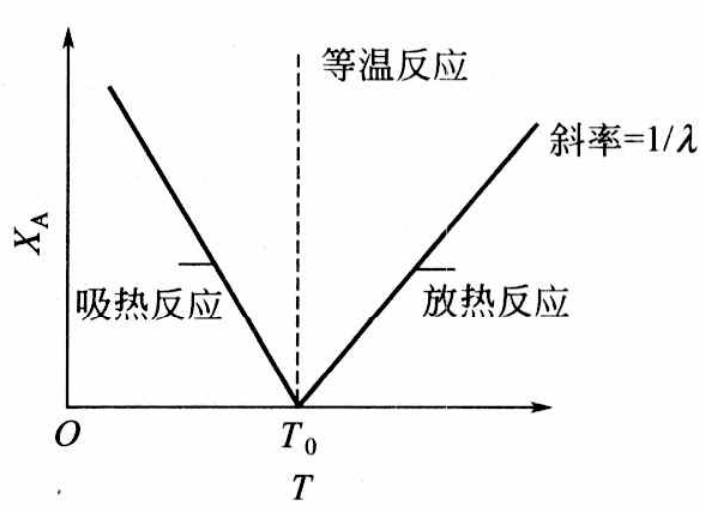
\includegraphics[width=\linewidth]{figs/fig4.7.png}
        \caption{绝热反应过程转化率与温度的关系}
        \end{figure}
    \end{minipage}\hfill
    \begin{minipage}{.48\linewidth}
        \begin{itemize}
            \item 该直线斜率为$1/\lambda$
            \item 放热反应，$\lambda>0$
            \item 吸热反应，$\lambda<0$
            \item 等温反应，$\lambda=0$
        \end{itemize}
    \end{minipage}

    \begin{itemize}
        \item 绝热条件下进行吸热反应时，反应温度随转化率的增加而下降
        \item 进行不可逆放热反应时，反应温度随转化率的增加而升高
    \end{itemize}

\end{frame}


\begin{frame}
    \frametitle{绝热管式反应器}

    \begin{minipage}{.48\linewidth}
        \begin{figure}            
        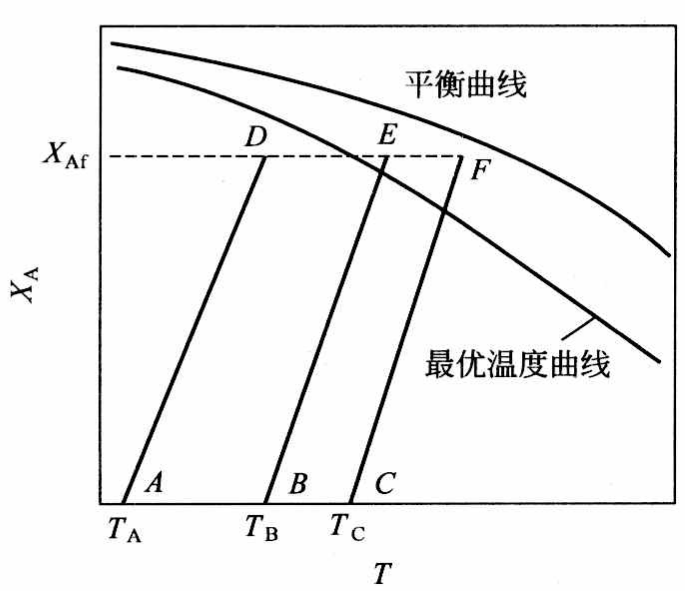
\includegraphics[width=\linewidth]{figs/fig4.8.png}
        \caption{可逆放热反应转化率与温度的关系}
        \end{figure}
    \end{minipage}\hfill
    \begin{minipage}{.48\linewidth}
        \begin{itemize}
            \item AD、BE、CF为不同进料温度下的绝热操作线。
            \item 对于一定的转化率，当反应温度低于最佳温度时，反应速率总是随温度的升高而增加，高于最佳温度时则随温度的升高而降低。
            \item 按BE线操作，其平均反应速率要大于AD线操作。
            \item 按CF线操作并不见得比BE线好，因为反应后期太接近平衡了，所以存在一最佳的进料温度。
        \end{itemize}
    \end{minipage}

\end{frame}


\begin{frame}
    \frametitle{绝热管式反应器的最佳的进料温度}

    \begin{minipage}{.35\linewidth}
        \begin{figure}            
        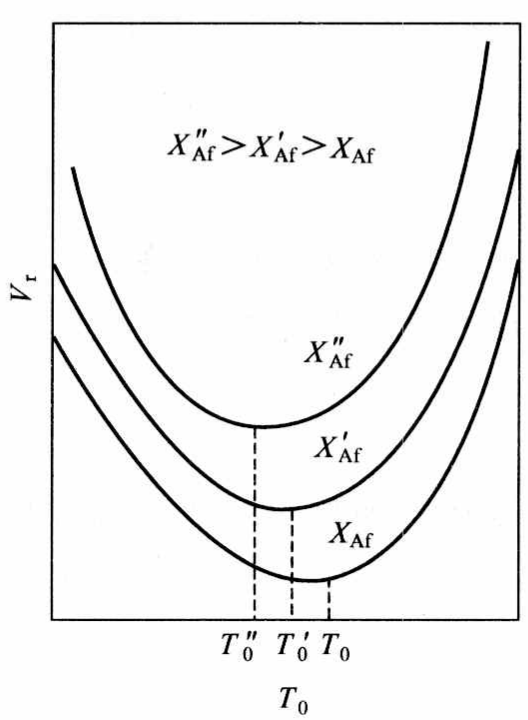
\includegraphics[width=\linewidth]{figs/fig4.9.png}
        \end{figure}
    \end{minipage}\hfill
    \begin{minipage}{.63\linewidth}
        \begin{itemize}
            \item 图中每条曲线是对一定的最终转化率而作出的
            \item 最终转化率越高，则最佳进料温度越低
            \item $X_\mathrm{AF}''>X_\mathrm{AF}'>X_\mathrm{AF}$，相应的最佳进料温度$T_0''<T_0'<T_0$
        \end{itemize}
    \end{minipage}

\end{frame}


\begin{frame}
    \frametitle{非绝热变温管式反应器}

    某些情况下，不适宜采用绝热操作
    \begin{itemize}
        \item 热效应很大的化学反应，绝热操作会使进出口物料温差太大
        \item 可逆放热反应，反应温度沿轴向升高，温度升高则平衡转化率降低，应用绝热反应器就得不到较高的转化率
        \item 可逆吸热反应，反应温度沿轴向降低，反应速率越来越慢
        \item 不可逆吸热反应，反应温度沿轴向降低，反应速率越来越慢，平衡转化率还会下降
        \item 由于某些原因，反应温度一定要控制在一定范围内的反应
            \begin{itemize}
                \item[\bullet] 温度过高会爆炸
                \item[\bullet] 温度过高会损坏催化剂
            \end{itemize}
    \end{itemize}
    这些情况下，在化学反应进行的同时必须与环境进行热交换

\end{frame}


\begin{frame}
    \frametitle{换热介质}

    常用高温换热介质
    \begin{itemize}
        \item 燃烧液体或气体燃料产生的烟道气
        \item 熔盐
        \item 高压蒸汽
    \end{itemize}
    常用低温换热介质
    \begin{itemize}
        \item 水
        \item 空气
        \item 反应原料
    \end{itemize}

\end{frame}


\begin{frame}
    \frametitle{列管式反应器}
    \begin{minipage}{0.68\linewidth}
        提高传热面积可采用列管式反应器，即将许多直径较小的管式反应器并联操作。
        \begin{enumerate}
          \item 提高传热面积
          \item 避免径向温差过大
        \end{enumerate}
        设计多管并联反应器时，一般可认为各管情况相同，所以只对一根管考察即能反应整个反应器的工况。
    \end{minipage}\hfill
    \begin{minipage}{0.28\linewidth}
        \begin{figure}[htpb]
            \centering
            
\includegraphics[width=\linewidth]{列管式反应器}
        \end{figure}
    \end{minipage}
    
\end{frame}